% Options for packages loaded elsewhere
\PassOptionsToPackage{unicode}{hyperref}
\PassOptionsToPackage{hyphens}{url}
%
\documentclass[
  10pt,
  a4paper,
]{article}
\usepackage{amsmath,amssymb}
\usepackage{iftex}
\ifPDFTeX
  \usepackage[T1]{fontenc}
  \usepackage[utf8]{inputenc}
  \usepackage{textcomp} % provide euro and other symbols
\else % if luatex or xetex
  \usepackage{unicode-math} % this also loads fontspec
  \defaultfontfeatures{Scale=MatchLowercase}
  \defaultfontfeatures[\rmfamily]{Ligatures=TeX,Scale=1}
\fi
\usepackage{lmodern}
\ifPDFTeX\else
  % xetex/luatex font selection
  \setmainfont[]{DejaVu Sans}
  \setmonofont[]{DejaVu Sans Mono}
\fi
% Use upquote if available, for straight quotes in verbatim environments
\IfFileExists{upquote.sty}{\usepackage{upquote}}{}
\IfFileExists{microtype.sty}{% use microtype if available
  \usepackage[]{microtype}
  \UseMicrotypeSet[protrusion]{basicmath} % disable protrusion for tt fonts
}{}
\makeatletter
\@ifundefined{KOMAClassName}{% if non-KOMA class
  \IfFileExists{parskip.sty}{%
    \usepackage{parskip}
  }{% else
    \setlength{\parindent}{0pt}
    \setlength{\parskip}{6pt plus 2pt minus 1pt}}
}{% if KOMA class
  \KOMAoptions{parskip=half}}
\makeatother
\usepackage{xcolor}
\usepackage[margin=19mm]{geometry}
\usepackage{longtable,booktabs,array}
\usepackage{calc} % for calculating minipage widths
% Correct order of tables after \paragraph or \subparagraph
\usepackage{etoolbox}
\makeatletter
\patchcmd\longtable{\par}{\if@noskipsec\mbox{}\fi\par}{}{}
\makeatother
% Allow footnotes in longtable head/foot
\IfFileExists{footnotehyper.sty}{\usepackage{footnotehyper}}{\usepackage{footnote}}
\makesavenoteenv{longtable}
\usepackage{graphicx}
\makeatletter
\def\maxwidth{\ifdim\Gin@nat@width>\linewidth\linewidth\else\Gin@nat@width\fi}
\def\maxheight{\ifdim\Gin@nat@height>\textheight\textheight\else\Gin@nat@height\fi}
\makeatother
% Scale images if necessary, so that they will not overflow the page
% margins by default, and it is still possible to overwrite the defaults
% using explicit options in \includegraphics[width, height, ...]{}
\setkeys{Gin}{width=\maxwidth,height=\maxheight,keepaspectratio}
% Set default figure placement to htbp
\makeatletter
\def\fps@figure{htbp}
\makeatother
\setlength{\emergencystretch}{3em} % prevent overfull lines
\providecommand{\tightlist}{%
  \setlength{\itemsep}{0pt}\setlength{\parskip}{0pt}}
\setcounter{secnumdepth}{-\maxdimen} % remove section numbering
\ifLuaTeX
\usepackage[bidi=basic]{babel}
\else
\usepackage[bidi=default]{babel}
\fi
\babelprovide[main,import]{french}
\ifPDFTeX
\else
\babelfont{rm}[]{DejaVu Sans}
\fi
% get rid of language-specific shorthands (see #6817):
\let\LanguageShortHands\languageshorthands
\def\languageshorthands#1{}
\usepackage{etoolbox}
\usepackage{microtype}
\usepackage{float}
\floatplacement{figure}{H}
\setlength{\emergencystretch}{3em}
\AtBeginEnvironment{longtable}{\small}
\ifLuaTeX
  \usepackage{selnolig}  % disable illegal ligatures
\fi
\IfFileExists{bookmark.sty}{\usepackage{bookmark}}{\usepackage{hyperref}}
\IfFileExists{xurl.sty}{\usepackage{xurl}}{} % add URL line breaks if available
\urlstyle{same}
\hypersetup{
  pdflang={fr-FR},
  hidelinks,
  pdfcreator={LaTeX via pandoc}}

\author{}
\date{}

\begin{document}

\hypertarget{v6.43---construire-des-ponts-avec-bellman}{%
\section{V6.43 - Construire des ponts avec
Bellman}\label{v6.43---construire-des-ponts-avec-bellman}}

\textbf{Document 67 · Vincent P. P. NOËL · 12 octobre 2026.} Preuves
auxiliaires et reconstruction de mécanismes classiques. Aucune nouveauté
historique ni preuve de RH revendiquée.

\hypertarget{le-diagnostic-une-fonction-de-valeur-trop-documentaire}{%
\subsection{1. Le diagnostic : une fonction de valeur trop
documentaire}\label{le-diagnostic-une-fonction-de-valeur-trop-documentaire}}

Le calcul V642 est exact pour sa fonction de valeur. Il explore toutes
les suites admissibles et conserve les ex aequo. Il n'est pas glouton et
n'utilise pas de facteur d'actualisation. Mais sa valeur terminale est
une couverture pondérée de tokens :

\[
U(D)=\sum_{t\in\bigcup_{a\in D}T_a}w_t,\qquad w_t\ge0.
\]

Cette fonction est sous-modulaire : si \(D\subset D'\), le gain d'une
action ajouté à \(D'\) est inférieur ou égal à son gain ajouté à \(D\).
En effet les nouveaux tokens sont \(T_a\setminus\bigcup_{b\in D}T_b\) ;
cet ensemble diminue lorsque \(D\) augmente. L'union empêche de compter
deux fois un acquis, mais ne représente pas une complémentarité positive
entre constructions.

Avec les cinq acquis V642 et les poids égaux, le budget 2 choisit le
rejeu DH et l'audit NB, gain 5. Après les audits, les extensions DH et
NB n'apportent chacune qu'un token nouveau pour un coût 3. Les nouveaux
ponts ne figurent pas dans l'ancien catalogue d'actions. Le défaut porte
donc sur les objets, la valeur et le catalogue, pas sur le principe de
Bellman.

\newpage

\begin{figure}
\centering
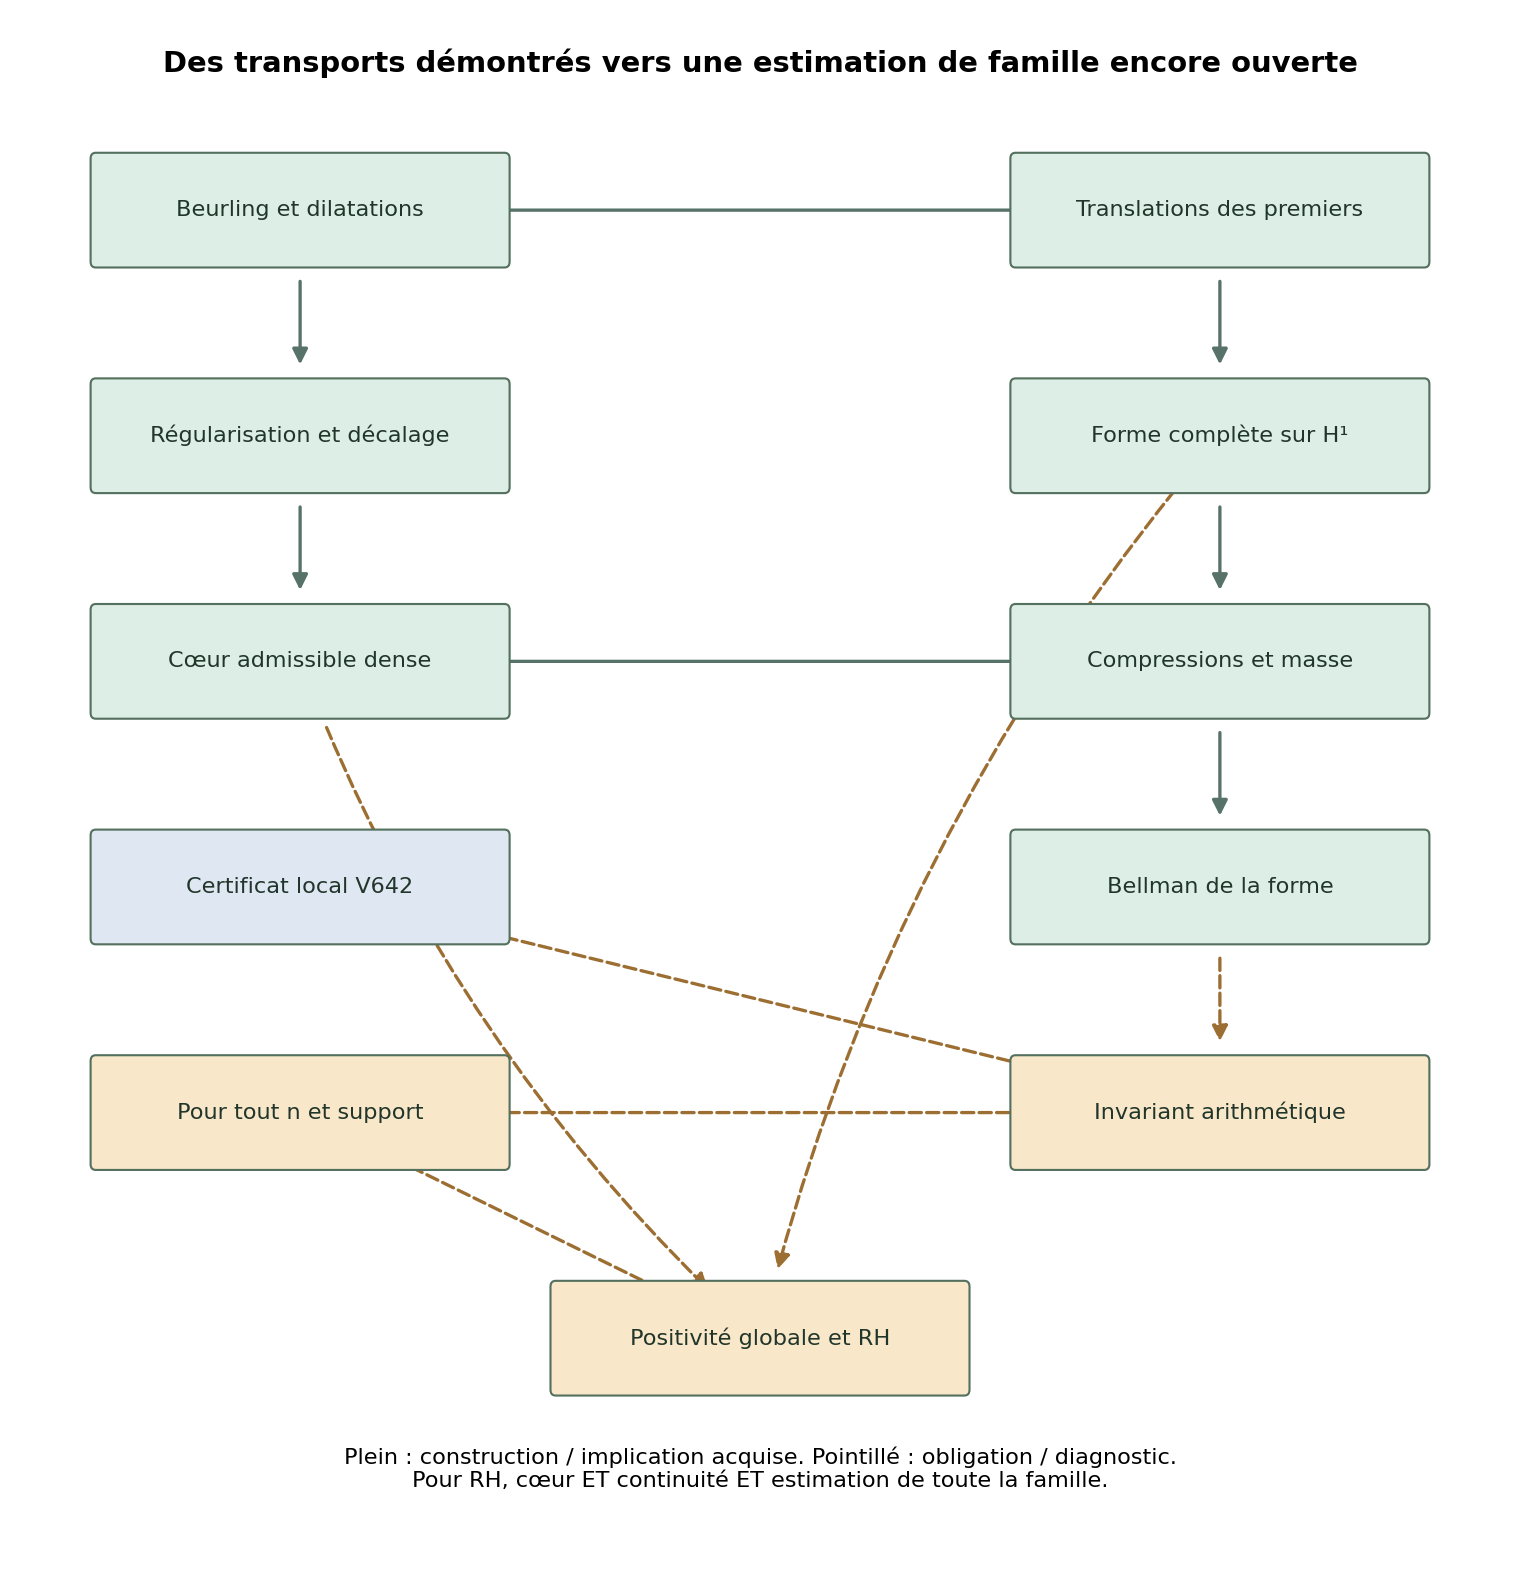
\includegraphics[width=0.9\textwidth,height=\textheight]{67_PONTS_ET_OBLIGATIONS.png}
\caption{Carte des constructions : les obligations ouvertes gardent leur
statut.}
\end{figure}

\newpage

\hypertarget{pont-b1---beurling-dilatations-mellin-et-translations}{%
\subsection{2. Pont B1 - Beurling, dilatations, Mellin et
translations}\label{pont-b1---beurling-dilatations-mellin-et-translations}}

Dans \(H=L^2(0,1)\), définir, pour \(0<\theta\le1\) et \(0<a\le1\),

\[
b_\theta(x)=\{\theta/x\}-\theta\{1/x\},\quad
D_af(x)=a^{-1/2}f(x/a)1_{(0,a)}(x).
\]

\(D_a\) est une isométrie ; ce n'est pas un opérateur unitaire sur cet
espace. L'application

\[
(Jf)(y)=e^{-y/2}f(e^{-y}),\qquad y>0
\]

est unitaire de \(H\) sur \(L^2(0,\infty)\) : le changement de variable
\(x=e^{-y}\) donne l'égalité des normes ; l'inverse est
\(f(x)=x^{-1/2}g(-\log x)\).

Pour \(a=e^{-t}\), \(t\ge0\), substitution directe donne

\[
JD_{e^{-t}}=R_tJ,\qquad
(R_tg)(y)=g(y-t)1_{(t,\infty)}(y).
\]

Le semi-groupe \(R_t\) est isométrique et son adjoint vaut
\(R_t^*g(y)=g(y+t)\). Directement, sur \(x<a\) puis sur \(x\ge a\),

\[
D_ab_\theta=a^{-1/2}(b_{a\theta}-\theta b_a).
\]

Ainsi la fermeture \(\mathcal N\) des combinaisons de \(b_\theta\) est
invariante par les dilatations. Si \(1\in\mathcal N\), alors
\(1_{(0,a)}=a^{1/2}D_a1\in\mathcal N\) ; les différences produisent les
indicatrices d'intervalles. Les fonctions en escalier étant denses,
\(\mathcal N=H\).

La formule de Mellin de la partie fractionnaire, d'abord intégrée pour
\(\Re s>1\), puis prolongée après cancellation du pôle, donne

\[
\mathcal Mb_\theta(s)=\int_0^1 b_\theta(x)x^{s-1}dx
=\frac{\zeta(s)}s(\theta-\theta^s),\qquad\Re s>0.
\]

Le point \(s=1\) est amovible dans le membre droit. Le membre gauche est
analytique dans \(\Re s>0\) car \(b_\theta\) est bornée. Pour
\(s=1/2+i\tau\), substitution donne la transformée de Fourier de
\(Jb_\theta\), avec convention \(e^{-i\tau y}\) ; les intégrales
convergent ici absolument. Pour un \(f\) général de \(L^2\),
l'identification sur la droite se comprend au sens de Plancherel.

Si \(\iota\) prolonge par zéro sur \(\mathbb R\), \(U_tg(x)=g(x-t)\) et
\(K_X\) est l'opérateur premier de V642, alors

\[
\iota R_t=U_t\iota,\qquad
\iota^*K_X\iota=\sum_{p^m\le X}\frac{\log p}{p^{m/2}}
(R_{m\log p}+R_{m\log p}^*).
\]

La seconde identité suit aussi pour les adjoints en comprimant
\(U_{-t}\). Ce transport est exact et indépendant de RH. Il rapproche
les représentations de Beurling et de la partie première de Weil ; il ne
fournit aucun signe. Le critère de Beurling, dans sa version \(p=2\),
identifie la densité précédente à RH {[}Beu55{]}. La fermeture est la
même que celle de sa classe à coefficients satisfaisant
\(\sum c_j\theta_j=0\) : une telle combinaison est une combinaison des
\(b_\theta\) ; réciproquement, si l'on exclut l'extrémité \(1\),
remplacer le second terme de \(b_\theta\) par \((\theta/r)\{r/x\}\),
\(r\to1^-\), donne des tests de cette classe qui convergent dans \(L^2\)
par convergence dominée.

\newpage

\hypertarget{pont-b2---une-forme-et-un-opuxe9rateur-construits-sans-supposer-le-signe}{%
\subsection{3. Pont B2 - Une forme et un opérateur construits sans
supposer le
signe}\label{pont-b2---une-forme-et-un-opuxe9rateur-construits-sans-supposer-le-signe}}

Fixer \(S>0\). Tout \(f\in H_0^1(-S,S)\) est prolongé par zéro, ce qui
donne un élément de \(H^1(\mathbb R)\). Poser

\[
h=f*f^*,\quad f^*(x)=\overline{f(-x)},\quad h(0)=\|f\|_2^2.
\]

Dans la convention Mellin V642 {[}CC21{]}, définir
\(Q_W=Q_{\rm arch}-Q_{\rm primes}\), avec

\[
Q_{\rm primes}(f)=2\sum_{p^m\le e^{2S}}\frac{\log p}{p^{m/2}}
\Re h(m\log p).
\]

Le support de \(h\) est contenu dans \([-2S,2S]\) : cette somme est
exactement finie. La formule archimédienne de V642 se réécrit

\[
Q_{\rm arch}(f)=\int_0^\infty w(x)\|U_xf-f\|_2^2dx-C_0\|f\|_2^2,
\quad w(x)=\frac{e^{-x/2}}{1-e^{-2x}},
\] \[
C_0=\log(8\pi)+\gamma_E+\pi/2.
\]

\textbf{Preuve de l'identité.} Utiliser \(h(-x)=\overline{h(x)}\) et
\(\|U_xf-f\|^2=2h(0)-2\Re h(x)\) dans la formule archimédienne. La
constante supplémentaire est \(2I\), où

\[
I=\int_0^\infty\frac{e^{-x/2}-e^{-x}}{1-e^{-2x}}dx
=2\int_0^1\frac{du}{(1+u)(1+u^2)}
=\frac\pi4+\frac{\log2}{2}.
\]

La dernière égalité suit de la décomposition
\(2/[(1+u)(1+u^2)]=1/(1+u)+(1-u)/(1+u^2)\). Les différences de
translations rendent l'intégrale convergente près de zéro. Fin de
preuve.

\textbf{Lemme de continuité.} La polarisation de \(Q_W\) définit une
forme hermitienne continue sur \(H_0^1(-S,S)\). Une constante explicite
admissible est

\[
M_S=A+B+C_0+2\sum_{p^m\le e^{2S}}\frac{\log p}{p^{m/2}},
\quad A=\frac1{2(1-e^{-2})},\quad B=\frac{8e^{-1/2}}{1-e^{-2}}.
\]

\textbf{Preuve.} Pour \(0<x<1\), \(\|U_xf-f\|_2\le x\|f'\|_2\) et
\(1-e^{-2x}\ge x(1-e^{-2})\). L'intégrale de \(w(x)x^2\) est au plus
\(A\). Pour \(x\ge1\), \(\|U_xf-f\|_2\le2\|f\|_2\) et
\(4\int_1^\infty w(x)dx\le B\). Ces mêmes majorants, appliqués aux
produits des différences de \(f,g\), contrôlent la forme polarisée.
Chaque corrélation première a module au plus \(\|f\|_2\|g\|_2\). Ainsi

\[
|Q_W(f,g)|\le M_S\|f\|_{H^1}\|g\|_{H^1}.
\]

Fin de preuve. La constante dépend de \(S\) ; aucune borne uniforme de
la partie première sur tout \(L^2\) n'est réintroduite.

Le sous-espace admissible

\[
E_S=\{f\in H_0^1(-S,S):\ell_+(f)=\ell_-(f)=0\},\quad
\ell_\pm(f)=\int f(x)e^{\pm x/2}dx,
\]

est fermé car les deux fonctionnelles sont continues. Munir \(E_S\) du
produit scalaire \textbf{externe}
\(\langle f,g\rangle_{H^1}=\int(\overline f g+\overline{f'}g')\). Le
théorème de Riesz appliqué à la forme continue donne un opérateur borné
autoadjoint \(T_S\) tel que \(Q_W(f,g)=\langle f,T_Sg\rangle_{H^1}\). Il
peut avoir un spectre négatif. Construire cet opérateur ne prouve donc
pas sa positivité ; son espace de Hilbert ne présuppose pas RH.

\newpage

\hypertarget{pont-b3---un-cux153ur-dense-et-le-quantificateur-qui-manque}{%
\subsection{4. Pont B3 - Un cœur dense et le quantificateur qui
manque}\label{pont-b3---un-cux153ur-dense-et-le-quantificateur-qui-manque}}

\textbf{Lemme du cœur.} \(C_c^\infty(-S,S)\cap E_S\) est dense dans
\(E_S\) pour la norme \(H^1\).

\textbf{Preuve.} Choisir une fonction paire \(\phi\ge0\), lisse, non
nulle, à support compact dans \((-S,S)\). Alors
\(\ell_+\phi=\ell_-\phi=c>0\) et, par intégration par parties,
\(\ell_\pm\phi'=\mp c/2\). Si \(g_n\in C_c^\infty\) converge vers
\(f\in E_S\), ses moments \(m_{n,\pm}\) tendent vers zéro. Poser

\[
a_n=(m_{n,+}+m_{n,-})/(2c),\quad
b_n=(m_{n,-}-m_{n,+})/c,
\quad v_n=g_n-a_n\phi-b_n\phi'.
\]

Alors \(\ell_\pm v_n=0\) et \(v_n\to f\) dans \(H^1\). Fin de preuve.

Le lemme G1 de V641 montre également que chaque test lisse admissible
s'écrit \(P\psi\), avec \(P=\partial_x^2-1/4\) et
\(\psi\in C_c^\infty(-S,S)\). Ce résultat peut être utilisé sans
supposer le signe de \(Q_W\).

Choisir une suite de tests \(v_j\) dont les sous-espaces emboîtés
\(V_n\) ont une union dense dans \(E_S\), et poser

\[
G_{S,n}=(Q_W(v_i,v_j))_{i,j\le n},\qquad
B_{S,n}=(\langle v_i,v_j\rangle_{H^1})_{i,j\le n}.
\]

Une base indépendante donne \(B_{S,n}>0\). C'est la métrique de masse ;
elle ne doit pas être remplacée par \(I\) sans orthonormalisation.

\textbf{Théorème de passage au domaine.} À \(S\) fixé, \(Q_W\ge0\) sur
\(E_S\) si et seulement si \(G_{S,n}\succeq0\) pour \textbf{tout} \(n\).
Plus généralement, des inégalités
\(G_{S,n}\succeq-\varepsilon_n B_{S,n}\) pour tout \(n\), avec
\(\varepsilon_n\to0\), suffisent.

\textbf{Preuve.} La nécessité est immédiate. Un \(v\in V_m\) appartient
à chaque \(V_n\), \(n\ge m\). Les inégalités avec erreur donnent
\(Q_W(v)\ge-\varepsilon_n\|v\|_{H^1}^2\) ; passer à la limite donne
\(Q_W(v)\ge0\). La densité et la continuité B2 étendent ensuite le signe
à \(E_S\). Fin de preuve.

Pour le critère global, il suffit de traiter chaque \(S\in\mathbb N^*\)
: tout test compact a son support dans l'un de ces intervalles. Aucun
majorant uniforme en \(S\) n'est nécessaire à cette implication logique.
En revanche, la preuve doit réellement couvrir chaque support et chaque
\(n\).

La vérification d'un nombre fini de matrices ne remplit pas ce
quantificateur. L'estimation sur une \textbf{famille entière} demeure le
travail ouvert ; le théorème ci-dessus l'identifie sans le résoudre.

\newpage

\hypertarget{pont-b4---ruxe9gulariser-et-transporter-une-erreur-avec-le-bon-duxe9calage}{%
\subsection{5. Pont B4 - Régulariser et transporter une erreur, avec le
bon
décalage}\label{pont-b4---ruxe9gulariser-et-transporter-une-erreur-avec-le-bon-duxe9calage}}

Les \(b_\theta\) ont des sauts. Une convergence NB dans \(L^2\) ne
contrôle pas directement \(Q_W\) dans \(H^1\). Prenons une mollifiante
\(\eta\in C_c^\infty(-1,1)\) d'intégrale 1,
\(\eta_\delta(x)=\delta^{-1}\eta(x/\delta)\), et
\(\chi\in C_c^\infty(-S,S)\).

Pour couvrir aussi les abscisses négatives, définir l'isométrie
\(\Gamma_S=U_{-(S+1)}\iota\). Puis

\[
\mathcal T_{S,\delta,\chi}g=P[\chi(\eta_\delta*\Gamma_Sg)].
\]

Cet opérateur envoie \(L^2(0,\infty)\) dans
\(C_c^\infty(-S,S)\cap E_S\). Les moments s'annulent par deux
intégrations par parties, car \(Pe^{\pm x/2}=0\).

Pour \(k\le3\), poser

\[
L_k=\sum_{j=0}^k\binom{k}{j}\|\chi^{(k-j)}\|_\infty
\delta^{-j}\|\eta^{(j)}\|_1,
\quad C_{S,\delta,\chi}=L_3+L_2+(L_1+L_0)/4.
\]

Young, Leibniz et l'isométrie de \(\Gamma_S\) donnent

\[
\|\mathcal Tg\|_{H^1}\le C_{S,\delta,\chi}\|g\|_2,
\quad C_{S,\delta,\chi}=O_\chi(\delta^{-3}),\quad0<\delta\le1.
\]

Par B2 et polarisation,

\[
|Q_W(\mathcal Tg)-Q_W(\mathcal Th)|
\le M_SC_{S,\delta,\chi}^2\|g-h\|_2(\|g\|_2+\|h\|_2).
\]

Ce contrôle est effectif à paramètres fixés, indépendamment de RH. Il
transporte une erreur ; il ne donne pas le signe des images.

\textbf{Couverture et limite.} Pour un \(\psi\in C_c^\infty(-S,S)\),
choisir \(\chi=1\) sur un voisinage de son support et
\(g_\psi(y)=\psi(y-S-1)\). Alors \(\Gamma_Sg_\psi=\psi\) et
\(\mathcal T g_\psi\to P\psi\) dans \(H^1\) lorsque \(\delta\to0\). Cela
suit de la convergence des mollifications dans \(H^3\). La réunion des
images, avec entrées \(L^2\) arbitraires, cutoffs et paramètres
variables, est donc dense dans \(E_S\), indépendamment de RH, par G1 et
le lemme du cœur. Une seule fonction \(\chi\) fixée ne couvre pas tous
les supports ; employer une famille de cutoffs ou un intervalle de
sortie plus large.

Sous l'hypothèse de densité NB, une diagonale avec
\(\|g_n-g_\psi\|_2=o(\delta_n^3)\) transporte cette approximation. Mais
la densité NB est elle-même équivalente à RH, et aucun signe des
approximants n'a été obtenu. Ce passage conditionnel ne peut servir de
preuve indépendante de RH.

\newpage

\hypertarget{pont-b5---bellman-sur-une-forme-la-dette-de-schur}{%
\subsection{6. Pont B5 - Bellman sur une forme : la dette de
Schur}\label{pont-b5---bellman-sur-une-forme-la-dette-de-schur}}

Considérer en dimension finie une forme hermitienne

\[
q(x,y)=x^*Ax+2\Re(x^*By)+y^*Cy.
\]

Si \(A>0\), compléter le carré donne

\[
q(x,y)=(x+A^{-1}By)^*A(x+A^{-1}By)
+y^*(C-B^*A^{-1}B)y.
\]

Donc \(\inf_x q(x,y)=y^*(C-B^*A^{-1}B)y\). C'est une vraie élimination
dynamique : la fonction de valeur restante est une forme quadratique, et
l'ajout ou l'élimination d'une variable modifie sa matrice par un
complément de Schur. L'infimum itéré est l'infimum conjoint ; aucune
récompense documentaire n'intervient.

Au passage d'une compression à la suivante,

\[
G_{n+1}=\begin{pmatrix}G_n&c_n\\c_n^*&a_n\end{pmatrix}.
\]

\textbf{Lemme de Schur singulier.} Cette matrice est positive
semi-définie si et seulement si

\[
G_n\succeq0,\quad c_n\in\operatorname{Ran}G_n,\quad
a_n-c_n^*G_n^\dagger c_n\ge0.
\]

\textbf{Preuve.} Si le grand bloc est positif, sa restriction \(G_n\)
l'est. Pour \(z\in\ker G_n\), faire varier \(x=tz\) à \(y\) fixé impose
\(z^*c_n=0\), donc la condition de portée. Lorsque \(G_nz=c_n\), le
carré complété reste valable avec ce \(z\) ; son terme résiduel est
\(a_n-c_n^*z\). Il est indépendant du choix de solution, égale
l'expression avec pseudo-inverse et doit être non négatif. La même
identité prouve la suffisance. Fin de preuve.

La quantité \(a_n-c_n^*G_n^\dagger c_n\) est la \textbf{dette de
couplage} à contrôler. Une famille arithmétique qui en prouverait le
signe pour tout \(n\), avec les conditions de noyau, ferait avancer la
preuve. La seule formule de Schur ne fournit pas cette estimation. En
dimension infinie ou sur un domaine non borné, les inverses et portées
demandent d'autres contrats : le lemme énoncé ici est fini.

Trois exemples rationnels synthétiques accompagnent le code :
\(G=[2],c=[1],a=1\) donne dette \(1/2\) ; \(G=[0],c=[1]\) échoue par
portée ; \(G=[2],c=[2],a=1\) donne dette \(-1\). Aucun de ces exemples
ne calcule une compression de zêta.

\newpage

\hypertarget{un-bellman-de-contrats-distinct-du-bellman-de-la-forme}{%
\subsection{7. Un Bellman de contrats, distinct du Bellman de la
forme}\label{un-bellman-de-contrats-distinct-du-bellman-de-la-forme}}

L'état du pilote est \((K,D,b)\) : faits et statuts \(K\), études
exécutées \(D\), budget restant \(b\). Chaque fait porte son domaine et
sa provenance. Un paquet AND exige toutes ses obligations ; plusieurs
paquets constituent des alternatives OR. Une étude peut produire un
candidat, sa réfutation précise, un obstacle de domaine ou une
estimation insuffisante. Son achèvement n'ajoute jamais automatiquement
le fait recherché.

Une capacité terminale est créditée une seule fois lorsque son contrat
est rempli :

\[
U(K)=\sum_B w_B1_{\{\exists j:\ C_{B,j}\subset K\}}.
\]

Le poids dépend du contrat, pas du nombre de fichiers. Une clarification
peut avoir une valeur déclarée ; elle garde un statut distinct d'un
théorème de signe. Les durées sont des intervalles
\([\tau_a^-,\tau_a^+]\) d'unités conventionnelles de travail.

Sans probabilités calibrées, deux enveloppes de scénarios sont calculées
:

\[
V_-(K,D,b)=\max\{U(K),\max_a\min_{o\in O_a}
V_-(K\cup K_{a,o},D\cup\{a\},b-\tau_a^+)\},
\]

et \(V_+\) emploie le maximum sur les issues et la durée basse. Les
actions doivent être admissibles et abordables ; STOP est toujours
autorisé. Les plans s'adaptent à l'issue obtenue. Par induction sur le
budget, la séparation entre STOP et premier choix prouve la récursion et
son optimalité dans ce modèle fini. Le budget diminue strictement ; les
actions ne se répètent pas.

Ces valeurs sont des enveloppes \textbf{du scénario déclaré}, pas des
intervalles de confiance empiriques. Le pessimisme peut privilégier
l'arrêt si toutes les issues sont inutiles. L'étude réelle peut coûter
davantage, et la liste des issues peut être incomplète. Aucune
probabilité de RH, aucune distance à RH et aucun apprentissage à partir
des anciennes fréquences n'est introduit.

Dans un exemple synthétique, deux constructions coûtent chacune 2 et
donnent ensemble une capacité de valeur 12 ; trois tâches locales
coûtent chacune 1 et donnent chacune 2. Au budget 4, Bellman choisit les
constructions et obtient 12, contre 6 pour les trois tâches. Cela
démontre le rôle de la complémentarité déclarée ; cela ne démontre pas
que les poids choisis conviennent à la recherche réelle.

Le modèle opérationnel V643 sépare les six lemmes acquis des issues
hypothétiques des futures études. Il ne peut créditer RH ou le signe
global par une transition. Les audits complets de candidats sont des
contrats de compréhension, pas des preuves positives. Le validateur
contrôle la structure et les faits réservés ; il ne vérifie pas
automatiquement les preuves ou la compatibilité de tous les domaines.
Les contrats restent relus dans le dossier.

\newpage

\begin{longtable}[]{@{}
  >{\raggedright\arraybackslash}p{(\columnwidth - 6\tabcolsep) * \real{0.2500}}
  >{\raggedright\arraybackslash}p{(\columnwidth - 6\tabcolsep) * \real{0.2500}}
  >{\raggedright\arraybackslash}p{(\columnwidth - 6\tabcolsep) * \real{0.2500}}
  >{\raggedright\arraybackslash}p{(\columnwidth - 6\tabcolsep) * \real{0.2500}}@{}}
\toprule\noalign{}
\begin{minipage}[b]{\linewidth}\raggedright
Budget H
\end{minipage} & \begin{minipage}[b]{\linewidth}\raggedright
Valeur basse U
\end{minipage} & \begin{minipage}[b]{\linewidth}\raggedright
Premiers choix bas
\end{minipage} & \begin{minipage}[b]{\linewidth}\raggedright
Valeur haute U
\end{minipage} \\
\midrule\noalign{}
\endhead
\bottomrule\noalign{}
\endlastfoot
2 & 0 & STOP & 3 \\
4 & 2 & Certifier un autre passage local à A fixé ; Terminer l'audit du
mémoire de Weil & 11 \\
6 & 3 & Chercher un invariant pour la dette de Schur & 16 \\
8 & 8 & Chercher un invariant pour la dette de Schur ; Construire une
famille régularisée et son défaut & 20 \\
10 & 11 & Chercher un invariant pour la dette de Schur ; Construire une
famille régularisée et son défaut & 22 \\
\end{longtable}

\hypertarget{unituxe9s-repruxe9sentation-et-duxe9cisions}{%
\subsection{8. Unités, représentation et
décisions}\label{unituxe9s-repruxe9sentation-et-duxe9cisions}}

Le logarithme arithmétique \(x\) reste sans dimension. Si
\([f]=\mathsf A\) est une unité fictive d'amplitude, alors
\([Q_W]=[\|f\|_{H^1}^2]=\mathsf E=\mathsf A^2\). \(T_S\), les
translations et les constantes normalisées sont sans dimension. Pour le
pilote, \([U]=[V]=\mathsf U\) et \([b]=[\tau]=\mathsf H\). Ces unités
rendent les calculs homogènes ; elles n'ajoutent aucun signe ni loi
physique.

La représentation imagée retenue est un pont dont les piliers sont le
domaine, le transport, l'estimation et les quantificateurs. Les arêtes
pleines représentent des implications démontrées ; la jonction vers RH
reste explicitement conditionnelle. Le graphe interactif expose les
hypothèses et les obstacles de chaque pilier.

\textbf{Prochaine construction prioritaire :} choisir une famille
admissible et écrire ses \(a_n,c_n,G_n\) depuis la forme arithmétique
complète ; proposer un invariant contrôlant la dette et les noyaux.
Avant un comptage massif, préciser la portée de l'invariant : tout
\(n\), tout support, ou seulement quelques blocs.

\textbf{Voie parallèle :} optimiser le défaut de régularisation et
choisir une métrique adaptée. Toute invocation de densité NB ou de
positivité de Weil doit garder son statut d'hypothèse équivalente à RH
lorsqu'elle sert d'entrée.

\textbf{Règle de fermeture :} un contre-exemple ferme le candidat et les
hypothèses effectivement testées ; une estimation absente laisse une
question ouverte. La fermeture du compagnon local V642 ne ferme ni
l'opérateur signé \(T_S\), ni toute la voie spectrale. Les certificats
locaux sont des instruments pour éprouver un mécanisme ; leur
multiplication ne remplit pas le quantificateur global.

\newpage

\hypertarget{sources-et-portuxe9e-de-la-lecture}{%
\subsection{Sources et portée de la
lecture}\label{sources-et-portuxe9e-de-la-lecture}}

{[}Beu55{]} A. Beurling, \emph{A closure problem related to the Riemann
zeta-function}, PNAS 41 (1955), 312-314 :
\href{https://www.pnas.org/doi/pdf/10.1073/pnas.41.5.312}{article
original}. Texte primaire relu ; les identités de transport et les
bornes de régularisation ci-dessus sont reconstruites et démontrées ici.

{[}CC21{]} A. Connes, C. Consani, \emph{Weil positivity and Trace
formula, the archimedean place} (2021) :
\href{https://alainconnes.org/wp-content/uploads/Selecta.pdf}{texte des
auteurs}. Introduction (4) et appendice B (149)-(151), normalisation
Mellin. Le résultat archimédien à support restreint n'est pas une
positivité globale incluant tous les premiers. Lecture ciblée, pas
validation intégrale du mémoire.

Weil 1948 : la lecture ciblée du théorème 10 et de l'application au
Frobenius dans la
\href{https://denisevellachemla.eu/Weil-courbes-varietes.pdf}{retranscription
du mémoire} corrige la fiche trop exclusivement centrée sur la
jacobienne. Le mémoire établit directement une positivité sur les
classes de correspondances. La lecture intégrale et le recoupement de la
retranscription avec l'édition restent ouverts.

Hamburger 1921 : original Math. Z. 10, 240-254, consulté dans le
\href{https://gdz.sub.uni-goettingen.de/download/pdf/PPN266833020_0010/PPN266833020_0010.pdf}{volume
original numérisé}. L'énoncé admet un nombre fini de pôles, une
croissance \(|f(s)|\le e^{|s|^\gamma}\) pour \(|s|\) assez grand, une
série de Dirichlet absolument convergente dans \(\Re s>1\) et l'équation
fonctionnelle exacte de zêta. La restriction au seul pôle 1 de la
présentation de Perelli est une version suffisante plus étroite. Cette
correction n'affaiblit pas les exigences d'identité de la fonction
recherchée.

Le double examen constructif et critique a conduit à corriger la
circularité possible du Hilbert de Weil, le défaut \(L^2/H^1\), le
décalage manquant de la demi-droite et la couverture des cutoffs. Il
s'agit d'une relecture interne, pas d'une expertise externe.

\end{document}
